\begin{figure}[b]
\vspace{-2mm}
    \centering
    \begin{subfigure}[c]{0.47\linewidth}
        \centering
        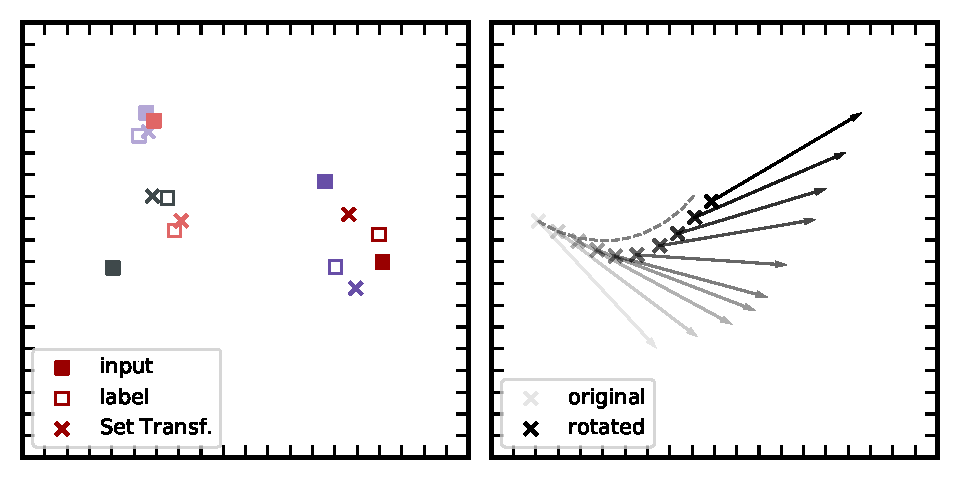
\includegraphics[width=\linewidth]{images/fig_nri_example_rotation_sett.pdf}
        \vspace{-6mm}
        \subcaption{Set Transformer}
        \label{fig:nri_rotation_example_A}
    \end{subfigure}
    % \hspace{mm}
    \hspace*{\fill}
    \begin{subfigure}[c]{0.47\linewidth}
        \centering
        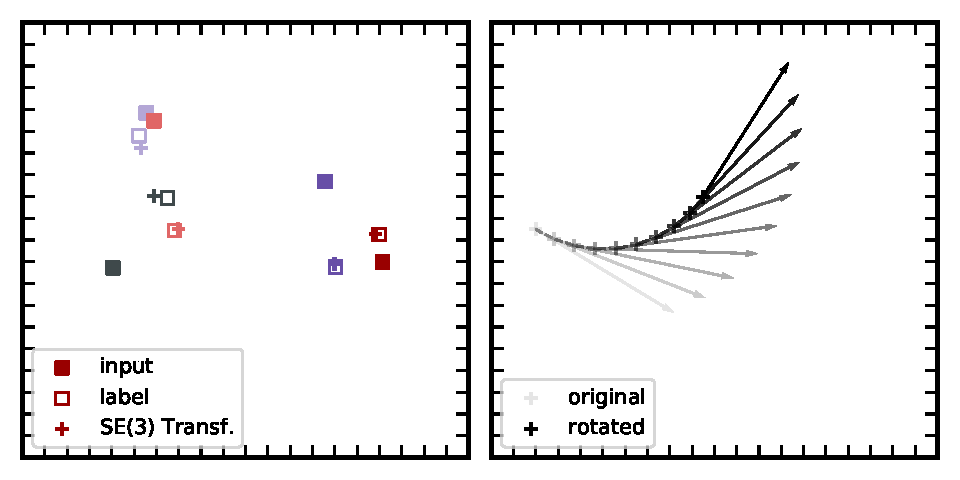
\includegraphics[width=\linewidth]{images/fig_nri_example_rotation_equi.pdf}
        \vspace{-6mm}
        \subcaption{SE(3)-Transformer}
        \label{fig:nri_rotation_example_B}
    \end{subfigure}
    \vspace{-1mm}
    \caption{A model based on conventional self-attention (left) and our rotation-equivariant version (right) predict future locations and velocities in a 5-body problem. The respective left-hand plots show input locations at time step $t=0$, ground truth locations at $t=500$, and the respective predictions. The right-hand plots show predicted locations and velocities for rotations of the input in steps of 10 degrees. The dashed curves show the predicted locations of a perfectly equivariant model.
    }
    \label{fig:nri_rotation_example}
\end{figure}
\section{Experiments}
We test the efficacy of the SE(3)-Transformer on three datasets, each testing different aspects of the model. The N-body problem is an equivariant task: rotation of the input should result in rotated predictions of locations and velocities of the particles. Next, we evaluate on a real-world object classification task. Here, the network is confronted with large point clouds of noisy data with symmetry only around the gravitational axis. Finally, we test the SE(3)-Transformer on a molecular property regression task, which shines light on its ability to incorporate rich graph structures. We compare to publicly available, state-of-the-art results as well as a set of our own baselines. Specifically, we compare to the Set-Transformer \citep{SetTransformer}, a non-equivariant attention model, and Tensor Field Networks \citep{ThomasSKYKR18}, which is similar to SE(3)-Transformer but does not leverage attention. 

Similar to \cite{Sosnovik20, Worrall19}, we measure the exactness of equivariance by applying uniformly sampled SO(3)-transformations to input and output. The distance between the two, averaged over samples, yields the equivariance error. Note that, unlike in \citet{Sosnovik20}, the error is not squared:
\begin{align}
    \Delta_{EQ}=\left\| L_{s} \Phi(f)-\Phi L_{s}(f)\right\|_{2} /\left\| L_{s} \Phi(f) \|_{2}\right.
\end{align}

\subsection{N-Body Simulations}

In this experiment, we use an adaptation of the dataset from \citet{KipfFWWZ18}. Five particles each carry either a positive or a negative charge and exert repulsive or attractive forces on each other. The input to the network is the position of a particle in a specific time step, its velocity, and its charge. The task of the algorithm is then to predict the relative location and velocity 500 time steps into the future. We deliberately formulated this as a regression problem to avoid the need to predict multiple time steps iteratively. Even though it certainly is an interesting direction for future research to combine equivariant attention with, e.g., an LSTM, our goal here was to test our core contribution and compare it to related models. This task sets itself apart from the other two experiments by not being invariant but equivariant: When the input is rotated or translated, the output changes respectively (see \Cref{fig:nri_rotation_example}).


We trained an SE(3)-Transformer with 4 equivariant layers, each followed by an attentive self-interaction layer (details are provided in the Appendix). \Cref{tab:RI} shows quantitative results. 
Our model outperforms both an attention-based, but not rotation-equivariant approach (Set Transformer) and a equivariant approach which does not levarage attention (Tensor Field). The equivariance error shows that our approach is indeed fully rotation equivariant up to the precision of the computations.



\begin{table}[]
{\caption{Predicting future locations and velocities in an electron-proton simulation.}
\label{tab:RI}}
\resizebox{\columnwidth}{!}{
\begin{tabular}{llrrrrr}
    \toprule
       &                     & Linear               & DeepSet \cite{Zaheer2017}              & Tensor Field \cite{ThomasSKYKR18}         & Set Transformer \cite{SetTransformer}      & \textbf{SE(3)-Transformer} \\
    %   &                     &                      & \cite{Zaheer2017}    &  \cite{ThomasSKYKR18}& \cite{SetTransformer}  &     \\
       \midrule
% \multicolumn{2}{l}{Position} & \multicolumn{1}{l}{} & \multicolumn{1}{l}{} & \multicolumn{1}{l}{} & \multicolumn{1}{l}{} & \multicolumn{1}{l}{}  \\
      & MSE $x$             & $0.0691$             & $0.0639$             & $0.0151$             & $0.0139$             & $\bm{0.0076}$              \\
       \textbf{Position} & std                 & -                    & $0.0086$             & $0.0011$             & $0.0004$             & $0.0002$              \\
       & $\Delta_{EQ}$       & -                    & $0.038$              & $1.9 \cdot 10^{-7}$  & $0.167$              & $3.2 \cdot 10^{-7}$   \\
       \midrule
% \multicolumn{2}{l}{Velocity} & \multicolumn{1}{l}{} & \multicolumn{1}{l}{} & \multicolumn{1}{l}{} & \multicolumn{1}{l}{} & \multicolumn{1}{l}{}  \\
      & MSE $v$             & $0.261$             & $0.246$              & $0.125$              & $0.101$              & $\bm{0.075}$              \\
       \textbf{Velocity} & std                 & -                    & $0.017$              & $0.002$              & $0.004$              & $0.001$               \\
       & $\Delta_{EQ}$       & -                    & $1.11$               & $5.0 \cdot 10^{-7}$  & $0.37$               & $6.3 \cdot 10^{-7}$   \\ 
       \bottomrule
% \label{tab:RI}
\end{tabular}}
\vspace{-3mm}
\end{table}





\subsection{Real-World Object Classification on ScanObjectNN}

\begin{figure}[t]
    \centering
    \begin{subfigure}[c]{0.45\linewidth}
        \centering
        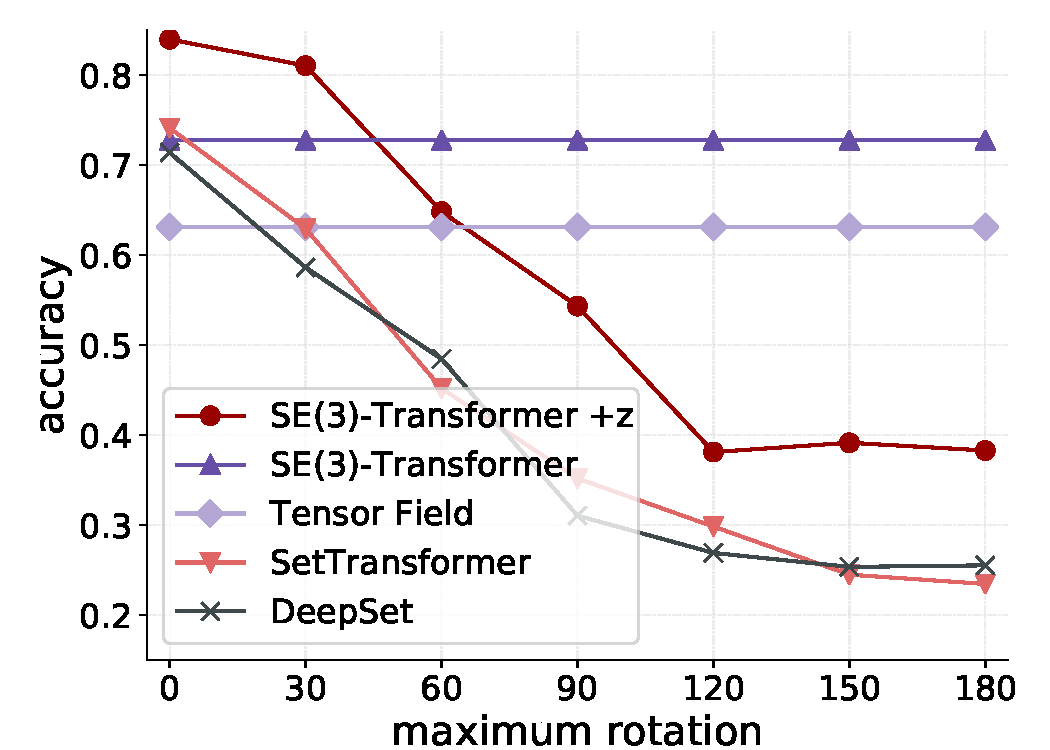
\includegraphics[width=\linewidth]{images/accuracy_over_angle.pdf}
        \subcaption{Training \textit{without} data augmentation.}
        \label{fig:scanobject_rotate_eval}
    \end{subfigure}
    \hspace*{\fill}
    \begin{subfigure}[c]{0.45\linewidth}
        \centering
        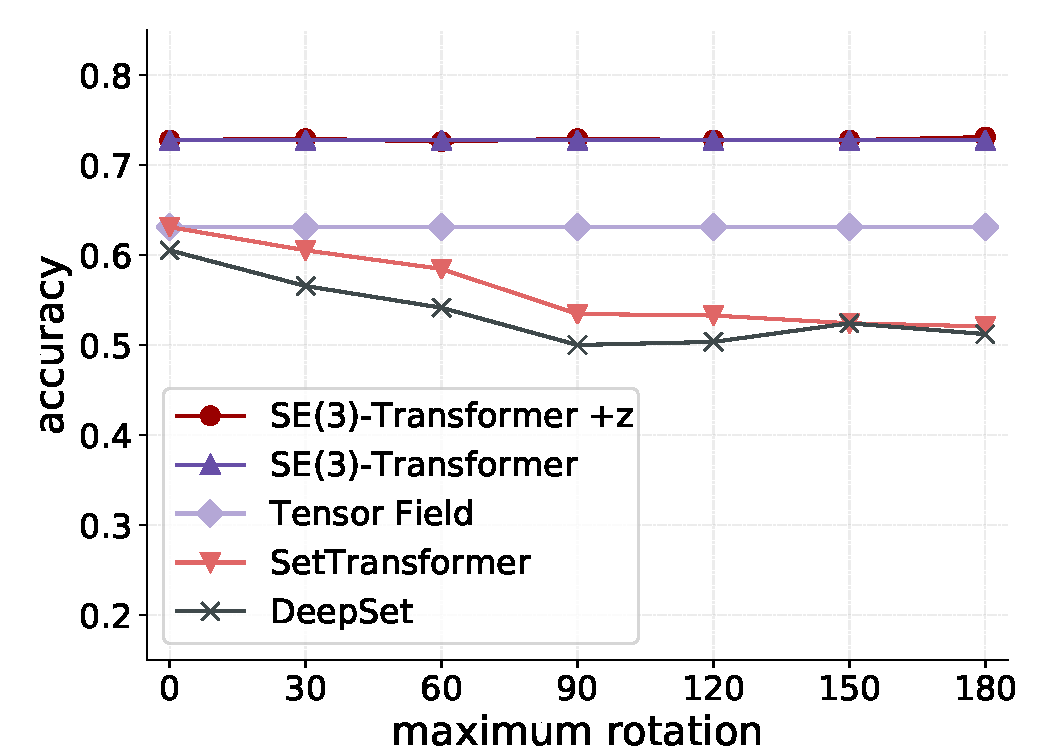
\includegraphics[width=\linewidth]{images/accuracy_over_angle_augmented.pdf}
        \subcaption{Training \textit{with} data augmentation.}
        \label{fig:scanobject_rotate_both}
    \end{subfigure}
    \caption{
        ScanObjectNN: $x$-axis shows data augmentation on the test set. The $x$-value corresponds to the maximum rotation around a random axis in the $x$-$y$-plane.
        If both training and test set are not rotated ($x=0$ in \textbf{a}), breaking the symmetry of the SE(3)-Transformer by providing the $z$-component of the coordinates as an additional, scalar input improves the performance significantly. Interestingly, the model learns to ignore the additional, symmetry-breaking input when the training set presents a rotation-invariant problem (strongly overlapping dark red circles and dark purple triangles in \textbf{b}).
    }
    \label{fig:scanobject_rotate}
\end{figure}

Object classification from point clouds is a well-studied task. Interestingly, the vast majority of current neural network methods work on scalar coordinates without incorporating vector specific inductive biases. Some recent works explore rotation invariant point cloud classification \cite{You2019,zhang2019rotation,ClusterNet,RaoFractal}. Our method sets itself apart by using roto-translation equivariant layers acting directly on the point cloud without prior projection onto a sphere \cite{RaoFractal,You2019,cohen2018spherical}. This allows for weight-tying and increased sample efficiency while transporting information about local and global orientation through the network - analogous to the translation equivariance of CNNs on 2D images. To test our method, we choose ScanObjectNN, a recently introduced dataset for real-world object classification. 
The benchmark provides point clouds of 2902 objects across 15 different categories. We only use the coordinates of the points as input and object categories as training labels. We train an SE(3)-Transformer with 4 equivariant layers with linear self-interaction followed by max-pooling and an MLP. Interestingly, the task is not fully rotation invariant, in a statistical sense, as the objects are aligned with respect to the gravity axis. This results in a performance loss when deploying a fully SO(3) invariant model (see \Cref{fig:scanobject_rotate_eval}). In other words: when looking at a new object, it helps to know where `up' is.
We create an SO(2) invariant version of our algorithm by additionally feeding the $z$-component as an type-0 field and the $x$, $y$ position as an additional type-1 field (see Appendix). We dub this model \textit{SE(3)-Transformer +z}. This way, the model can `learn' which symmetries to adhere to by suppressing and promoting different inputs (compare \Cref{fig:scanobject_rotate_eval} and \Cref{fig:scanobject_rotate_both}). In \Cref{tab:Scan}, we compare our model to the current state-of-the-art in object classification\footnote{At time of submission, PointGLR was a recently published preprint \citep{PointGLR}. The performance of the following models was taken from the official benchmark of the dataset as of June 4th, 2020 (\url{https://hkust-vgd.github.io/benchmark/}): 3DmFV \citep{3dmfv}, PointNet \citep{Pointnet}, SpiderCNN \citep{SpiderCNN}, PointNet++ \citep{Pointnetpp}, DGCN \citep{DGCNN}.}. Despite the dataset not playing to the strengths of our model (full SE(3)-invariance) and a much lower number of input points, the performance is competitive with models specifically designed for object classification - PointGLR \citep{PointGLR}, for instance, is pre-trained on the larger ModelNet40 dataset \citep{modelnet40}. For a discussion of performance vs. number of input points used, see \Cref{sec:app_n_points}.


\begin{table}[t]
\vspace{-1mm}
{\caption{Classification accuracy on the 'object only' category of the ScanObjectNN dataset\textsuperscript{4}. The performance of the SE(3)-Transformer is averaged over 5 runs (standard deviation 0.7\%).}
\label{tab:Scan}}
\centering
% for rotating text, see bottom of page:
% https://tex.stackexchange.com/questions/98388/how-to-make-table-with-rotated-table-headers-in-latex
% \mcrot{1}{l}{60}{\twoelementtable{DeepSet}{\cite{Zaheer2017}}} 
\resizebox{0.98\columnwidth}{!}{
\vspace{2mm}
\begin{tabular}{lrrrrrrrrrrrrr}
\toprule
 & \mcrot{1}{l}{30}{Tensor Field} & \mcrot{1}{l}{30}{DeepSet} & \mcrot{1}{l}{30}{\textbf{SE(3)-Transf.}} & \mcrot{1}{l}{30}{3DmFV} & \mcrot{1}{l}{30}{Set Transformer} & \mcrot{1}{l}{30}{PointNet} & \mcrot{1}{l}{30}{SpiderCNN} & \mcrot{1}{l}{30}{Tensor Field +z} & \mcrot{1}{l}{30}{PointNet++} & \mcrot{1}{l}{30}{\textbf{SE(3)-Transf.+z}} & \mcrot{1}{l}{30}{PointCNN} & \mcrot{1}{l}{30}{DGCNN} & \mcrot{1}{l}{30}{PointGLR}\\
% \vspace{1mm}
\midrule
\vspace{1mm}
No. Points & 128 & 1024 & \textbf{128} & 1024 & 1024 & 1024 & 1024 & 128 & 1024 & \textbf{128}  & 1024  & 1024  & 1024 \\
\vspace{1mm}
Accuracy & 63.1\% & 71.4\% & \textbf{72.8} \% & 73.8\% & 74.1\% & 79.2\% & 79.5\% & 81.0\% & 84.3\% & \textbf{85.0\%} & 85.5\% & 86.2\% & 87.2\% \\
\bottomrule
\end{tabular}
}
\vspace{-2mm}
\end{table}

\newpage
\subsection{QM9}

\begin{wraptable}[10]{R}{0.65\linewidth} %[Zeilenhöhe]{Ausrichtung}[Überhang]{Breite}
\vspace{-8mm}
{\caption{QM9 Mean Absolute Error. Top: Non-equivariant models. Bottom: Equivariant models. SE(3)-Tr. is averaged over 5 runs.}
% \vspace{-1mm}
\label{tab:QM9}}
\resizebox{0.65\columnwidth}{!}{
\begin{tabular}{lrrrrrr}
    \toprule
    \textsc{Task}   & $\alpha$ & $\Delta \varepsilon$ & $\varepsilon_\text{HOMO}$ & $\varepsilon_\text{LUMO}$ & $\mu$ & $C_\nu$ \\
    \textsc{Units}  & $\text{bohr}^3$ & meV & meV & meV & D & cal/mol K  \\
    \midrule 
    WaveScatt~\citep{HirnMP17}   & .160  & 118   & 85    & 76    & .340  & .049  \\
    NMP~\citep{Gilmer2017}        & .092  & 69    & 43    & 38    & .030  & .040   \\
    SchNet~\citep{schnet}     & .235  & 63    & 41    & 34    & .033  & .033   \\
    \midrule
    Cormorant~\cite{anderson2019cormorant}   & .085  & 61    & 34    & 38    & .038  & .026 \\
    LieConv(T3)~\citep{Finzi2020} & .084 & 49   & 30   & 25    & .032  & .038 \\
    TFN~\citep{ThomasSKYKR18} & .223  & 58    & 40    & 38    & .064  & .101 \\
    \textbf{SE(3)-Transformer}          & .142$\pm$.002  & 53.0$\pm$0.3    & 35.0$\pm$.9    & 33.0$\pm$.7    & .051$\pm$.001  & .054$\pm$.002 \\
    \bottomrule
\end{tabular}
}
\end{wraptable}


The QM9 regression dataset \citep{RamakrishnanDRvL14} is a publicly available chemical property prediction task. There are 134k molecules with up to 29 atoms per molecule. Atoms are represented as a 5 dimensional one-hot node embeddings in a molecular graph connected by 4 different chemical bond types  (more details in Appendix). `Positions' of each atom are provided. We show results on the test set of \citet{anderson2019cormorant} for 6 regression tasks in \Cref{tab:QM9}. Lower is better. The table is split into non-equivariant (top) and equivariant models (bottom). Our nearest models are Cormorant and TFN (own implementation). We see that while not state-of-the-art, we offer competitive performance, especially against Cormorant and TFN, which transform under irreducible representations of SE(3) (like us), unlike LieConv(T3), using a left-regular representation of SE(3), which may explain its success.

